\begin{savequote}
\quoteperson{For most of my life, one of the persons most baffled by my 
  own work was myself.}{Beno\^it Mandelbrot}
\end{savequote}

\chapter{Generating Fractals using Geometric Algebra}
\label{chap:fractals}

In this chapter we investigate ways that a number of classical, well know
fractals may be generated using Geometric Algebra. Further we show how
GA can be used to form a natural generalisation to higher dimensions and
well known fractals may be generated using Geometric Algebra. Further we show
how GA can be used to form a natural generalisation to higher dimensions and
non-Euclidean geometries. Some rendering strategies will also be discussed.

Fractals have always been a popular topic in computer graphics due to their
ability to give rise to great \ae sthetic beauty from a relatively simple
mathematical description. Generally a fractal is considered to be any
geometric object which possesses detail on all
scales\cite{FRAC:FractalsEverywhere, FRAC:FractalGeometryOfNature}. That is to
say, one may examine the edge of the object under arbitrary magnification
yet still find it rough and irregular. Many introductions to the subject of
fractals and their creation on computers exist elsewhere\cite{FRAC:FractalGeometry,
  FRAC:ChaosAndFractals, FRAC:FractalImages}.

The term fractal was coined by Mandelbrot\cite{FRAC:LesObjetsFractals} in 1975,
originally from the Latin {\em fractus} (broken) intended as a way of referring
to their edges which looks like jagged cracks in some surface. Since many
fractals (particularly those arising from so-caled \emph{Iterated Function Systems}) have
fractional Hausdorff dimension\cite{FRAC:GeometryOfFractalSets},
some have joked that `fractal' is actually a portmanteau word formed from
`fractionally' and `dimensional'.

Below we shall investigate an extension, via GA, of the class of fractals 
which is most associated with Mandelbrot -- those based on repeated iteration
of a complex function.  Similar fractals have found applications in a wide
selection of research areas including image 
compression\cite{Barnsley88c,Barnsley93b}.% and
%antenna design\cite{FRAC:Antennas}. 
It is hoped that the GA-based approach here may
also be of use in a similar manner however in this chapter we concentrate more
on the \ae sthetic nature of the fractals.

\section{Fractals from Complex Iteration}

\begin{figure}
\centering
\begin{tabular}{c@{$\quad$}c}
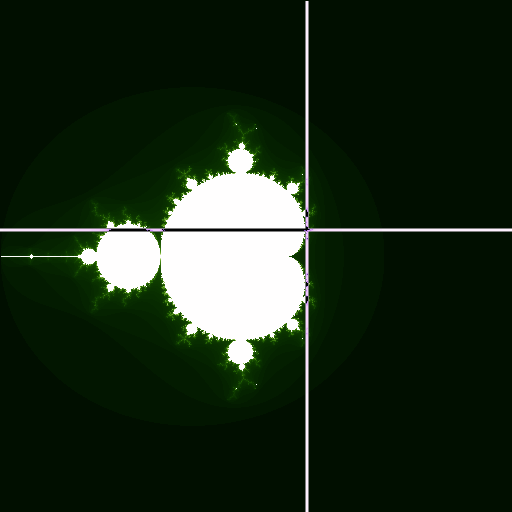
\includegraphics[width=0.4\textwidth]{euc_mandel_julia_pos} 
 & 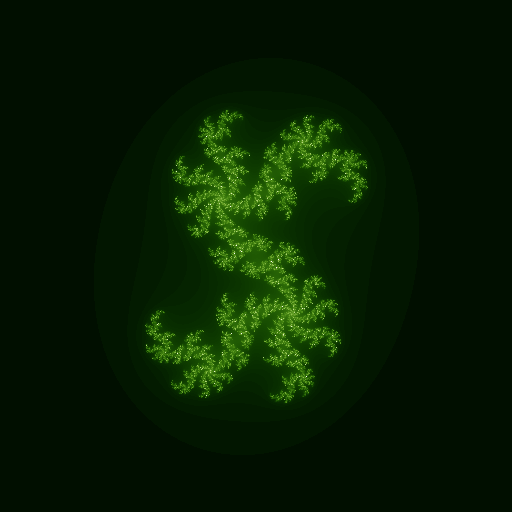
\includegraphics[width=0.4\textwidth]{julia_euc} \\
                          (a) & (b)
\end{tabular}
\caption{\label{fig:euclidean_sets}The well known (a) Mandelbrot set with
  the constant $c = 0.4 + 0.2i$ marked and (b) the Julia
  set associated with $c$.}
\end{figure}

The classical Mandelbrot and Julia sets (figure \ref{fig:euclidean_sets}) are
well known, even to laymen, as examples of fractals. They are
examples of a form of fractal known as \emph{recurrence} or 
\emph{escape-time}
fractals.  Such fractals are generated by iterating some complex function and
noting how fast it `escapes' to infinity (if at all).

Both fractals are displayed by mapping points in the complex plane to
pixels in the final image.
Usually this mapping to an image pixel location $\mathbf{x} = [\; x\;y \;]^T$
from its corresponding complex number, $c$, is simple.

\begin{definition}[Representation of the Complex Plane]
An image point $\mathbf{x} = [\; x\;y \;]^T$ is mapped to a point on the 
complex plane via that mapping $\mathbf{x} \mapsto {\mathcal I}(x)$ where
\[
{\mathcal I}({\mathbf x}) = [\; a_1 x + b_1 \; a_2 y + b_2 \;]^T
\]
and $(b_1,b_2)$ specify the origin of the area of interest in the complex
plane and $(a_1,a_2)$ specify its scale.
%\[
%{\mathcal I}(x) = [\; 1 \; i \;] \left[ 
%  \begin{array}{ccc}
%a & 0 & c \\
%0 & b & d \\
%  \end{array}
%\right]
%\left[
%  \begin{array}{c}
%  \mathbf{x} \\ 1
%  \end{array}
%\right].
%\]
%where constants $a,b,c$ and $d$ are set so as to specify 
%the area of the complex 
%plane shown in the image.
\end{definition}

The same complex function generates both the Mandelbrot and
Julia sets\cite{FRAC:Mandelbrot, FRAC:JuliaMandelBook}. It is worth noting
that other functions could be used and hence many other escape-time fractals
exist. In this chapter, to save space, we shall only consider developments from this function.

\begin{definition}
The complex function $f(z)$, $c \in {\mathbb C}$,
    is defined as
\[
f(z) = z^2 + c.
\]
\end{definition}

\begin{definition}[Iteration]
Iteration of a function $f(x)$ is denoted as $f^{(n)}(z)$ where
\[
f^{(n)}(z) \equiv f(f^{(n-1)}(z))
\]
and $f^{(0)}(z) \equiv z$, $n \in {\mathbb Z}^+$.
\end{definition}

\subsection{The Mandelbrot Set}

\begin{definition}[The Mandelbrot set]
The Mandelbrot set, $\mathbb{M}$, is defined as
\[
\mathbb{M} = 
\left\{c \in \mathbb{C} 
: \lim_{n \rightarrow \infty} \magof{f^{(n)}(0)} < \infty \right\} 
\]
where $\magof{z} \equiv (zz^*)^\frac{1}{2}$.
\end{definition}

\begin{lemma} 
\label{lem:convergence}
If $\magof{f^{(n)}(x)} \ge 2$
for some $n$ and $x$ then $\magof{f^{(n)}(x)} \rightarrow \infty$ as $n
\rightarrow \infty$.
\begin{proof}Suppose 
$\magof{f^{(n)}(x)} > 2$ and $\magof{f^{(n)}(x)} > \magof{c}$. It is
clear that
\[
\frac{\magof{f^{(n+1)}(x)}}{\magof{f^{(n)}(x)}} =
\frac{\magof{f^{(n)}(x)^2 + c}}{\magof{f^{(n)}(x)}}
\]
and hence
\[
\frac{\magof{f^{(n+1)}(x)}}{\magof{f^{(n)}(x)}} \ge 
\frac{\magof{f^{(n)}(x)}^2 - \magof{c}}{\magof{f^{(n)}(x)}} =
\magof{f^{(n)}(x)} - \frac{\magof{c}}{\magof{f^{(n)}(x)}}.
\]
As $\magof{f^{(n)}(x)} > \magof{c}$ and $\magof{f^{(n)}(x)} > 2$ then
\[
\magof{f^{(n)}(x)} - \frac{\magof{c}}{\magof{f^{(n)}(x)}} >
\magof{f^{(n)}(x)} - 1 > 1
\]
giving
\[
\frac{\magof{f^{(n+1)}(x)}}{\magof{f^{(n)}(x)}} \ge 1
\]
implying $\magof{f^{(n)}(x)} \rightarrow \infty$ as $n
\rightarrow \infty$ as required.
\end{proof}
\end{lemma}

Using lemma \ref{lem:convergence} we may determine if some point $x$ is
\emph{not} in the set as soon as $\magof{f^{(n)}(x)} \ge 2$.  In practise one
may have to wait an arbitrarily long time for this condition to be met and one
will never obtain it if $x$ is within the set. We approximate the set by
choosing some maximum number of iterations to wait before labelling $x$ as
being within the set.  Our algorithm for generating an image of the set is
shown in algorithm \ref{alg:generate_mandelbrot}.

\begin{fancyalg}
\begin{algorithmic}[1]
\STATE $i_{\mathrm{max}} :=$ maximum number of iterations
\FORALL{points $\mathbf{x}$ in image}
\STATE $c := {\mathcal I}(\mathbf{x})$
\STATE $z := c$
\STATE $i := 0$
\WHILE{$zz^* < 4$ and $i < i_{\mathrm{max}}$}
  \STATE $z := z^2 + c$
  \STATE $i := i+1$
\ENDWHILE 
\STATE set pixel $\mathbf{x}$ to colour $i$
\ENDFOR
\end{algorithmic}
\caption{
\label{alg:generate_mandelbrot}
  Generating the Mandelbrot set}
\end{fancyalg}

The level of detail of the resulting image being determined by the value of $i_{\mathrm{max}}$.
The image of the Mandelbrot set in figure \ref{fig:euclidean_sets}a was
generated with $\mathbf{x} = [\;x\;y\;]^T, x \in (-2,2), y \in (-2,2)$.
In figure \ref{fig:euclidean_sets}a a colour palette was also chosen such that colour 0 was black
and colour $i_{\mathrm{max}}$ was white moving through dark-green. The brightness of
each pixel is therefore some measure of how long it took to decide whether that point was
a member of the set.

\subsection{The Julia Set}

There are an infinite number of Julia sets; each point on the complex plane
has a corresponding Julia set. The definition of the Julia set is somewhat
similar to that of the Mandelbrot set.

\begin{definition}[The Julia set]
The Julia set, $\mathbb{J}_c$, associated
with the complex number $c$ is given by
\[
\mathbb{J}_c = 
\left\{z \in \mathbb{C}
: \lim_{n \rightarrow \infty} \magof{f^{(n)}(z)} < \infty \right\}.
\]
\end{definition}

The difference between this and the Mandelbrot set is that there exists a 
Julia set associated with each complex number, $c$ which must be chosen before
generating the image. Our algorithm for generating Julia sets is, as one would
expect, similar to that for the Mandelbrot set and is shown in algorithm
\ref{alg:generate_julia}.

\begin{fancyalg}
\begin{algorithmic}[1]
\REQUIRE{$c =$ constant}
\STATE $i_{\mathrm{max}} :=$ maximum number of iterations
\FORALL{points $\mathbf{x}$ in image}
\STATE $z := {\mathcal I}(\mathbf{x})$
\STATE $i := 0$
\WHILE{$zz^* < 4$ and $i < i_{\mathrm{max}}$}
  \STATE $z := z^2 + c$
  \STATE $i := i+1$
\ENDWHILE 
\STATE set pixel $x$ to colour $i$
\ENDFOR
\end{algorithmic}
\caption{
\label{alg:generate_julia}
  Generating the Julia set}
\end{fancyalg}

Due to their similarity, there exist a number of theorems and conjectures which link the
Mandelbrot and Julia sets in some way. For example, if $c \in \mathbb{M}$ then
the Julia set $\mathbb{J}_c$ is connected\cite{FRAC:JuliaAndMandelbrotSets}.
If $c$ is near the border of $\mathbb{M}$ then it is a Cantor
set\cite{FRAC:JuliaAndMandelbrotSets}.

\section{Extending Complex Numbers}

In this section we will seek to find a co-ordinate free analogue to the
complex mapping $z \mapsto z^2$ in order to re-cast the fractals above in
terms of geometric operations using GA. We will start by confining ourselves
to the plane and then move into higher dimensions.

Firstly we define a mapping between the complex numbers, $\mathbb{C}$, and
the vector-space of the complex plane, $\mathbb{R}^2$. Letting $\{e_1, e_2\}$
be some orthonormal basis for $\mathbb{R}^2$ we can form a natural one-to-one
mapping between $r \in \mathbb{R}^2$ and $C(r) \in \mathbb{C}$:

\begin{definition}
Given some vector $r \in \mathbb{R}^2$, we can map one-to-one into the
complex plane by forming the complex number
\[
C(r) = (r \cdot e_1) + (r \cdot e_2)i.
\]
\end{definition}

Here it is clear that $e_1$ corresponds to the real-axis and $e_2$ 
corresponds to the imaginary axis of the complex plane.
By squaring we have
\begin{align*}
[C(r)]^2 &= [(r \cdot e_1) + (r \cdot e_2)i]^2 \\
       &= (r \cdot e_1)^2 - (r \cdot e_2)^2 + 2(r \cdot e_1)(r \cdot e_2)i.
\end{align*}
%which is analogous to the usual method of squaring complex numbers.

\begin{lemma}
Given some vector $r \in \mathbb{R}^2$ representing the complex number
$C(r)$, the mapping $r \mapsto re_1r$ is equivalent to $C(r) \mapsto [C(r)]^2$.
\end{lemma}
\begin{proof}
Let $r = xe_1 + ye_2$. Therefore $C(r) = x + yi$. It is clear that
\begin{align*}
re_1r &= (x^2 - y^2) e_1 + 2xye_2 \\
\Rightarrow\;C(re_1r) &= (x^2 - y^2) + 2xyi\\
        &= [C(r)]^2
\end{align*}
as required.
\end{proof}

%To complete the extension one must also define a geometric equivalent of
%addition:
Complex addition is identical to vector addition using this representation.
\begin{lemma}
Given vectors $r, c \in \mathbb{R}^2$ representing the complex numbers
$C(r)$ and $C(c)$, the mapping $r \mapsto r + c$ is equivalent to 
$C(r) \mapsto C(r) + C(c)$.
\end{lemma}
\begin{proof}
Clear by direct substitution.
\end{proof}

\section{Moving to Higher Dimensions}

In this section we extend the mapping above to more than two spatial dimensions.
This turns out to be remarkably easy since the mapping is co-ordinate free;
we simply remove the constraint that the vectors need be in $\mathbb{R}^2$.

\begin{definition}
Given a vector $r$ and some unit basis vector $e_1$ the mapping
$r \mapsto re_1r$ is the geometric analogue of squaring a complex number.
\end{definition}

Vector addition can once again be used in place of complex addition.

%\begin{definition}
%Given two vectors, $r$ and $c$, the geometric analogue of complex addition
%is $r \mapsto r + c$.
%\end{definition}

We may now define generalised Mandelbrot and Julia sets based upon
a new vector recurrence relation.

\begin{definition}\label{def:gen_f(r)}
The vector analogue of $f(r)$ is 
\[
f_v(r) = re_1r + c
\]
with initial values being defined by a particular fractal.
\end{definition}

\subsection{The Generalised Mandelbrot Set}

We can now reformulate the definition of the Mandelbrot set in a co-ordinate
free, dimension agnostic manner. Our new algorithm is shown in figure
\ref{alg:generalised_mandelbrot} and we may define the generalised
Mandelbrot set similarly to the Mandelbrot set. Referring back to lemma
\ref{lem:convergence} we see that the argument we used to terminate the iteration
when $\magof{f^{(n)}(x)} \ge 2$ still holds when we use $\magof{x} = \sqrt{x \cdot x}$.

\begin{definition}[The generalised Mandelbrot set]
The generalised Mandelbrot set, $\mathbb{M}_k$, in $\mathbb{R}^k$ 
    is defined as
\[
\mathbb{M}_k = 
\left\{c \in \mathbb{R}^k 
: \lim_{n \rightarrow \infty} f_v^{(n)}(0) < \infty \right\}.
\]
\end{definition}

\begin{fancyalg}
\begin{algorithmic}[1]
\REQUIRE{Set $\mathcal I$ of vectors associated with image points}
\STATE $i_{\mathrm{max}} :=$ maximum number of iterations
\STATE $e_1 :=$ a unit vector in some preferred direction
\FORALL{$c \in {\mathcal I}$}
\STATE $r := c$
\STATE $i := 0$
\WHILE{$r^2 < 4$ and $i < i_{\mathrm{max}}$}
  \STATE $r := re_1r + c$
  \STATE $i := i+1$
\ENDWHILE 
\STATE set pixel $c$ to colour $i$
\ENDFOR
\end{algorithmic}
\caption{
\label{alg:generalised_mandelbrot}
  Generating the Generalised Mandelbrot set}
\end{fancyalg}

\begin{figure}
\centering
\begin{tabular}{c@{$\quad$}c}
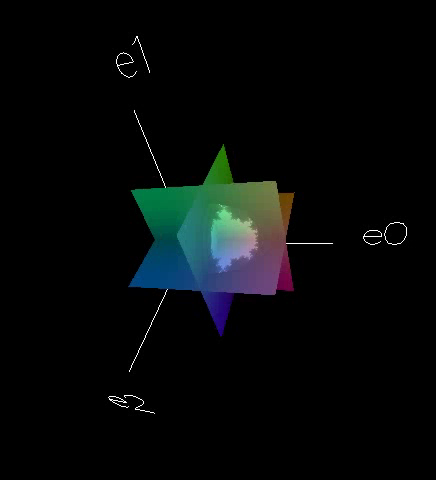
\includegraphics[width=0.4\textwidth]{3dmandel1}
 & 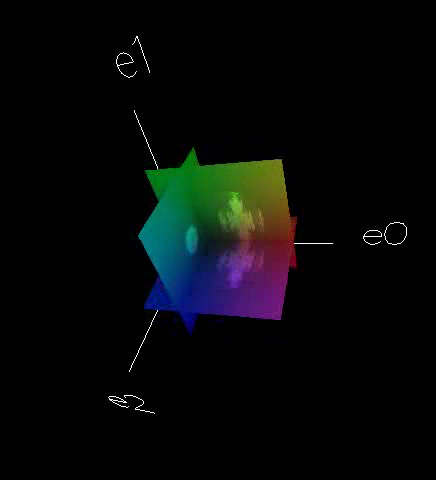
\includegraphics[width=0.4\textwidth]{3dmandel2} 
\end{tabular}
\caption{\label{fig:3dmandel}
  Two frames from an animation showing slices through
          the 3 dimensional Mandelbrot set.}
\end{figure}

%Since we are no longer restricted to the complex plane we may choose many ways
%to associate an image plane point $(x,y)$ with a corresponding constant
%vector $c$. 

In figure \ref{fig:3dmandel} vectors lying in three orthogonal
planes were used to generate three images of the three-dimensional
Mandelbrot set which are then displayed mapped onto the original planes. This
gives a crude visualisation method. A better method used to generate pictures
of the generalised Julia set is given below.

The method used was to render a number of slices through the set leaving transparent the points in
each slice which were not a part of the fractal. These slices were then stacked
atop each other to give the impression of a three dimensional surface as illustrated
in figure \ref{fig:voxel}.

\subsection{The Generalised Julia Set}

\begin{figure}
\centering
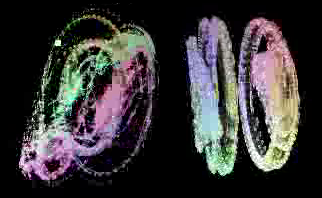
\includegraphics[width=0.8\textwidth]{3djulia_pair}
\caption{\label{fig:3djulia}
  Two frames from an animation showing voxel
          rendering of 3d Julia sets.}
\end{figure}

We may generalise the Julia set in an analogous manner and generate it
using algorithm \ref{alg:generalised_julia}.

\begin{definition}[The generalised Julia set]
The generalised Julia set, $\mathbb{J}_{c,k}$, in $\mathbb{R}^k$
which is associated with the vector $c \in \mathbb{R}^k$ is given by
\[
\mathbb{J}_{c,k} = 
\left\{x \in \mathbb{R}^k
: \lim_{n \rightarrow \infty} f_v^{(n)}(x) < \infty \right\}.
\]
\end{definition}

\begin{fancyalg}
\begin{algorithmic}[1]
\REQUIRE{Set $\mathcal I$ of vectors associated with image points}
\REQUIRE{$c =$ constant vector}
\STATE $i_{\mathrm{max}} :=$ maximum number of iterations
\STATE $e_1 :=$ a unit vector in some preferred direction
\FORALL{$r \in {\mathcal I}$}
\STATE $i := 0$
\WHILE{$r^2 < 4$ and $i < i_{\mathrm{max}}$}
  \STATE $r := re_1r + c$
  \STATE $i := i+1$
\ENDWHILE 
\STATE set pixel $r$ to colour $i$
\ENDFOR
\end{algorithmic}
\caption{
\label{alg:generalised_julia}
  Generating the Generalised Julia set}
\end{fancyalg}

\begin{figure}
\centering
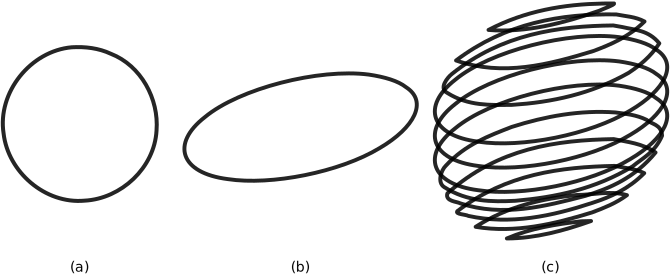
\includegraphics[width=0.8\textwidth]{voxel}
\caption{\label{fig:voxel}
  A crude form of voxel rendering. (a) A specific slice through the set. (b) Viewed from
  an oblique angle. (c) Stacked with other slices giving the impression of a three
  dimensional shape.
}
\end{figure}

Figure \ref{fig:3djulia} was rendered using a crude form of voxel rendering. A
number of 2-dimensional 'slices' were rendered at varying heights in the set. Each
pixel was coloured, or left transparent, depending on whether it was within or without
the set. Finally, each slice was rendered at an oblique angle. The resulting
`stack' of slices gave an approximation to the true shape. Figure
\ref{fig:voxel} illustrates this process.

The voxel rendering was adequate to visualise the fractals and confirm the algorithm
works, but a more sophisticated rendering technique is desirable which can generate
sharper images.

\subsection{Ray Tracing}

In this section we briefly extend the method in \cite{FRAC:HypercomplexIterations} of 
ray-tracing quaternionic escape-time fractals to the generalised GA fractals developed 
above. Ray-tracing of fractals is achieved by finding some distance function
$d(x;\Omega)$ which gives the minimum distance to the fractal parameterised by
$\Omega$ along the from the point $x$. For a Julia fractal the
parameter $\Omega$ is the constant we have previously termed $c$. For a Mandelbrot fractal there is no
parameter as the fractal is unique. 

In \cite{FRAC:HypercomplexIterations} it was shown, for the complex number
form of the escape time fractals above, that such a distance function
at a point $z$ in the complex plane $d_z$ was bounded by
\[
d_z > \lim_{n \rightarrow \infty}\,\frac{|z_n|}a{2|z'_n|}\log|z_n|
\]
where $z_n = z_{n-1}^2 + c$, $|z'_n| = 2|z_{n+1}||z'_{n+1}|$, $z'_0 = 0$.
The values of $z_0$ and $c$ were dictated by the type of fractal as described above.

It was found that extending the formula to vectors using our analogue of
complex multiplication yielded a suitable distance function although this has not
yet been formally proved. Specifically
\[
d(x; \Omega) = \lim_{n \rightarrow \infty}\,\frac{|x_n|}a{2|x'_n|}\log|x_n|
\]
where $x_n = f_v(x_{n-1})$, $|x'_n| = 2|x_{n+1}||x'_{n+1}|$, $x'_0 = 0$ and
the initial value of $x_n$ is fractal dependant. 

Once a distance function (or a lower bound thereof) is available ray tracing
becomes possible. Rays of light are traced back from point in the image
plane of an imaginary camera to the scene. For a particular ray the algorithm
to trace the fractal is as follows.

\begin{enumerate}
\item Set $\hat{r}$ to be a unit vector pointing along the ray direction.
\item Set the current position, $x$, to be the camera origin.
\item Calculate a lower bound, $d_-$ for the distance from $x$. 
\item If $d_-$ is smaller than some tolerance $\tau$ exit reporting
$x$ as the intersection point with the fractal.
\item Set $x \leftarrow x + d_-\hat{r}$.
\item Go to step 3.
\end{enumerate}

\begin{figure}
\centering
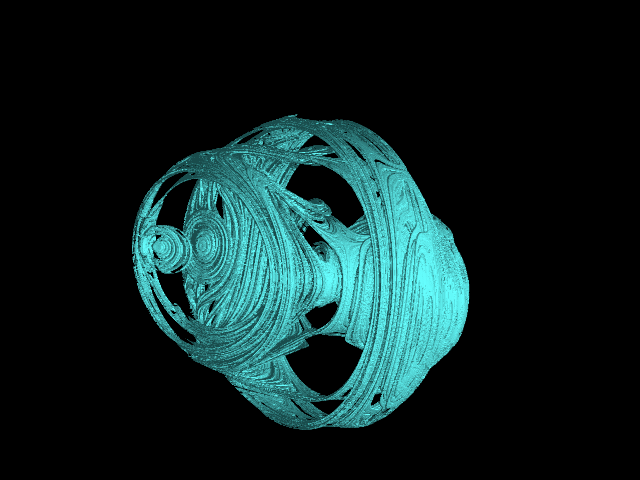
\includegraphics[width=0.8\textwidth]{5djulia}
\caption{\label{fig:5djulia}
  A ray-traced three-dimensional slice through a five-dimensional Julia set.
}
\end{figure}

Once the intersection point is found the fractal may be lit by examining
intersection points of neighbouring rays and taking the surface orientation
to be that of a plane passing through the neighbouring intersection points.
Figure \ref{fig:5djulia} shows a slice through a 5d Julia set rendered with
this technique.

\section{Moving to Hyperbolic Geometry}

So far all our fractals have been generated using the Euclidean geometry of
the complex plane or $n$-dimensional flat space. In this section we
extend our algorithm using the non-Euclidean tools
given to us by conformal GA. We firstly need to re-define our complex function
in terms of the geometric operations.

Viewed using Euclidean geometry our function $f(r)$ firstly reflects and
scales the vector $r \mapsto re_1r$ and then translates via the vector $c$. We
know already how to translate using conformal GA so we turn our attention to
the former operation.

Since we constructed our GA approach to be analogous to the complex number approach we
may borrow the geometric interpretation from complex numbers. In this case the mapping 
$r \mapsto r^2$ acts to rotate r by $\mathrm{arg}(r)$ and scale it by
$\magof{r}$. We may therefore extend this interpretation into our GA solution as in
figure \ref{fig:rotate}. We firstly work only in the $r \wedge e_1$ plane to allow
our analogy with complex numbers to hold. If $\theta$ is the angle between $r$ and
$e_1$, i.e.
\[
\theta = \cos^{-1}\left(\frac{r \cdot e_1}{\magof{r}}\right),
\] 
then the mapping $r \mapsto re_1r$ is initially a rotation in the plane $r \wedge e_1$
by $\theta$ followed by a dilation by a factor of $(r^2)^\frac{1}{2}$ 
which may be expressed in terms of rotors and dilators using their geometric
definitions above.

\begin{definition}
The conformal GA analogue of $r \mapsto re_1r$ is given by
\[
F(re_1r) = D_r R_r\,F(r)\,\tilde{R}_r \tilde{D}_r
\]
where
\begin{eqnarray*}
R_r & = & \cos \frac{\theta}{2} + P \sin \frac{\theta}{2},
    \quad
P = \frac{(r \wedge e_1)}{\magof{r}}
\end{eqnarray*}
and $\theta$ is defined above.
The dilator $D_r$ acts to dilate about the origin by a factor of
$\magof{r}$. In Euclidean geometry it is given by
\[
D_r = \exp\left( \frac{-\log(\magof{r})}{2} e\bar{e} \right).
\]
\end{definition}

\begin{figure}
\centering
\includegraphics[width=0.5\textwidth]{rotate}
\caption{\label{fig:rotate}%
  The geometrical interpretation of $r \mapsto re_1r$ as a rotation followed by a dilation.
}
\end{figure}

The second part of $f(r)$ is a translation by $c$. A translator in non-Euclidean
geometries is only defined as translating the origin to a given point so we must be
careful about the precise operations we perform. The GA analogue of the
complex mapping $r \mapsto r + c$ is thus given by the following steps:
\begin{enumerate}
\item Translate $r$ to the origin by applying the appropriate geometry-specific translator represented by $\tau(-r)$;
\item Translate the origin to $c$ by applying the translator $\tau(c)$;
\item `Undo' step 1 by applying the translator $\tau(r)$.
\end{enumerate}
where $\tau(r)$ is a function which will give the appropriate translator for our 
chosen geometry. In Euclidean geometry $\tau(r) = 1 + \frac{nr}{2}$ and in
non-Euclidean geometry
\[
\tau(r) = \frac{1}{\sqrt{\lambda^2 - r^2}}(\lambda + \bar{e}r)
\]
with $\lambda$ being defined as in the discussion of non-Euclidean geometries above.

A little thought will reveal that this is equivalent to translating $c$ by the translator
$1 + \frac{nr}{2}$. We may therefore define our full conformal GA analogue of $f(r)$.

\begin{definition}
The conformal GA analogue of $f(r) = re_1r + c$ is given by
\[
f(r) = F^{-1}(T_r F(c) \tilde{T}_r)
\]
where
\[
T_r = \tau(F^{-1}(D_r R_r\,F(r)\,\tilde{R}_r \tilde{D}_r))
\]
\end{definition}

\begin{figure}[p]
\centering
\begin{tabular}{c}
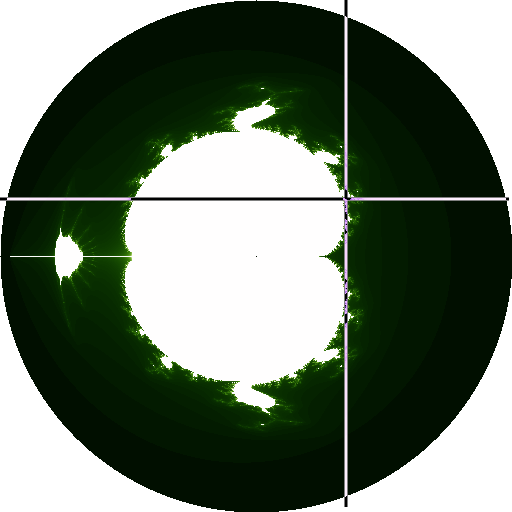
\includegraphics[width=0.35\textheight]{hyp_mandel_julia_pos} \\ (a) \\
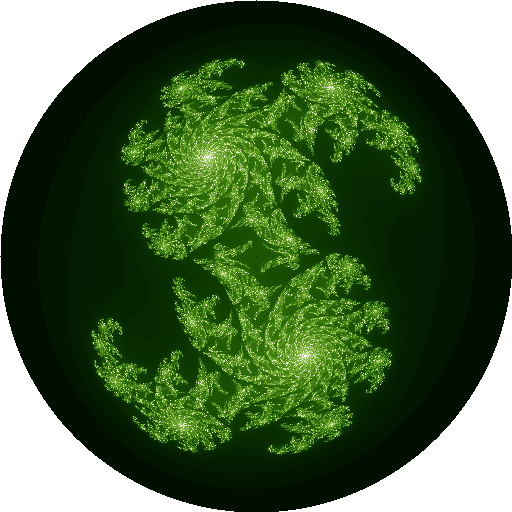
\includegraphics[width=0.35\textheight]{julia_hyp} \\
                          (b)
\end{tabular}
\caption{\label{fig:noneuclidean_sets}The non-Euclidean analogue of the (a) Mandelbrot set with
  the constant $c = 0.4e_1 + 0.2e_2$ marked and (b) the Julia
  set associated with $c$.}
\end{figure}

Our algorithm for generating the generalised Mandelbrot and Julia sets is now identical
except we substitute our new, geometric, definition of $f(r)$ and choose $\tau(r)$
and the form of $D_r$ to reflect our chosen geometry. Usefully pure-rotation rotors remain
the same in each geometry so no modification of them is necessary. Figure
\ref{fig:noneuclidean_sets} shows a hyperbolic Mandelbrot and Julia set on the
Poincar\'e disc generated with this method. 

\subsection{The Hyperbolic Mandelbrot Set}

The hyperbolic Mandelbrot set is shown in figure \ref{fig:noneuclidean_sets}a and
is generated using algorithm \ref{alg:generalised_mandelbrot}, substituting
step 7 for one performing the iteration outlined above. 

\subsection{The Hyperbolic Julia Set}

A particular hyperbolic Julia set is shown in figures \ref{fig:noneuclidean_sets}b,
\ref{fig:julia_montage} and \ref{fig:julia_montage2}.  Once again, it is generated using algorithm
\ref{alg:generalised_julia} substituting step 6. The two related montage figures show the same path
across the underlying Mandelbrot set but with two differing methods of representing
$x \mapsto x+c$. It is interesting to note that not only are the fractals different but they have different
overall shape and behaviour. It is also worth remarking that, geometrically, there is no preferred form
of the translation representation and so both these montages are equally valid images of hyperbolic Julia sets.
This leads to the interesting conclusion that, whilst there is only one family of Euclidean Julia sets, for
transitionally non-commuting geometries there are two.

\begin{figure}[p]
\centering
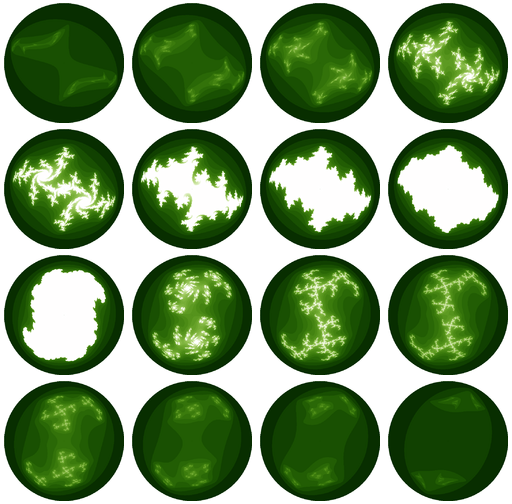
\includegraphics[width=0.9\textwidth]{julia_montage}
\caption{\label{fig:julia_montage} 
  A montage of hyperbolic Julia sets where the constant $c$ moves from $-0.7e_1 - 0.7e_2$
  to $0.7e_1 + 0.7e_2$. 
  In this figure translation $x \mapsto x + c$ is performed by applying a
  translation rotor corresponding to $c$ to the vector $x$.
}
\end{figure}

\begin{figure}[p]
\centering
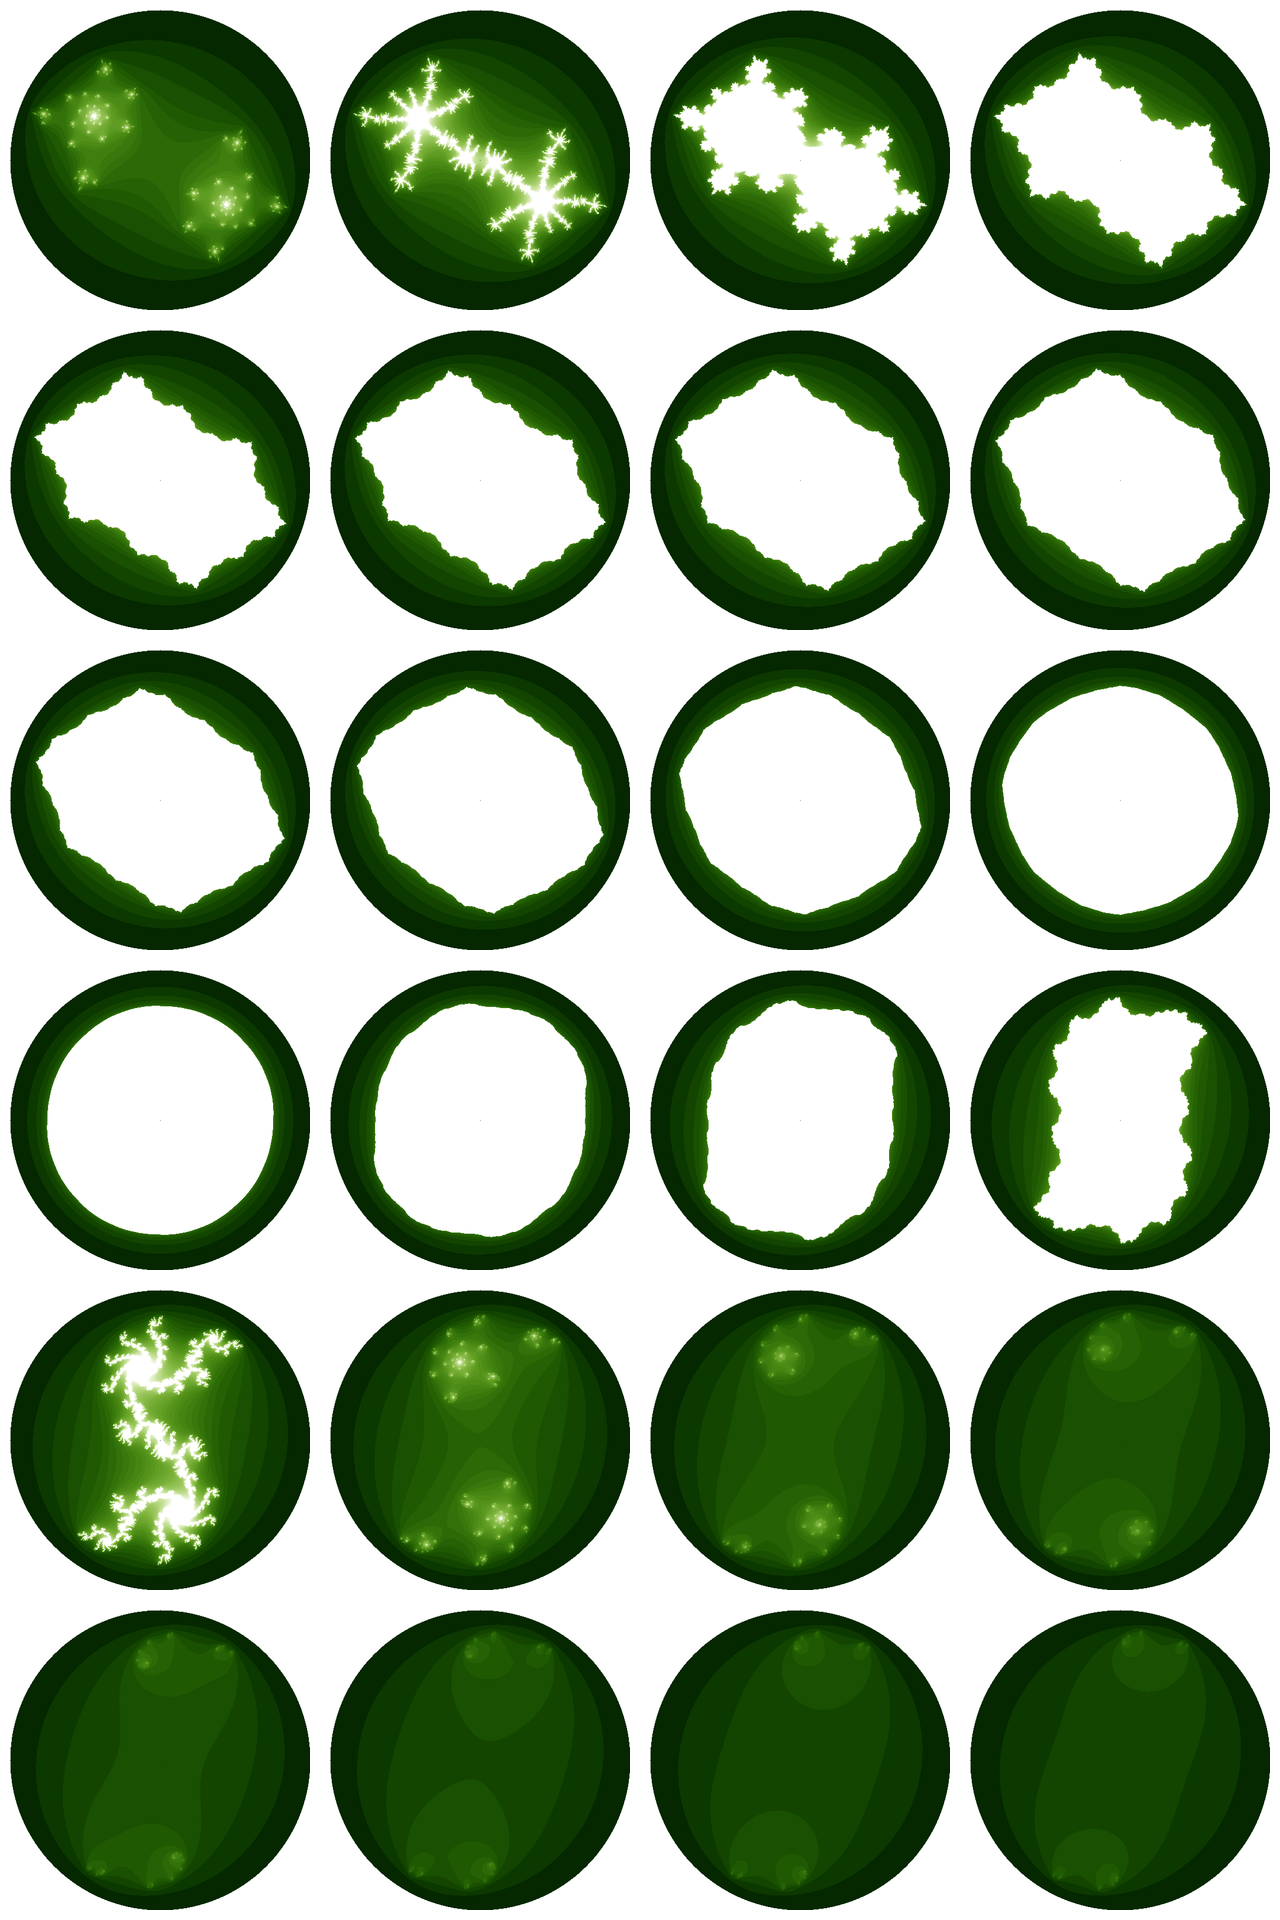
\includegraphics[width=0.9\textwidth]{direct_julia_noneuclid}
\caption{\label{fig:julia_montage2}
  A montage of hyperbolic Julia sets where the constant $c$ moves from $-0.7e_1 - 0.7e_2$
  to $0.7e_1 + 0.7e_2$. 
  In this figure translation $x \mapsto x + c$ is performed by applying a
  translation rotor corresponding to $x$ to the vector $c$.
}
\end{figure}

It is worth noting that the code to generate the Euclidean fractals in figure 
\ref{fig:euclidean_sets} is identical to that used to generate
\ref{fig:julia_montage} except for the definition of translators and dilators.
We can replace the Euclidean form with those given in section
\ref{sec:extendconfmodel} and re-cast the fractals into hyperbolic geometry.
The fact that conformal GA algorithms developed using Euclidean geometry may
so readily be applied to non-Euclidean geometries by simply changing the rotor
definitions neatly indicates the power of the conformal GA approach.



